\subsection{Basic Algorithm}

In our protocol, a peer first tries to download the file from an origin web server.  If at some point one of the following conditions occurs, the download will switch to a peer-to-peer swarming download:
\begin{enumerate}
\item First the client waits a maximum amount of time $T$ after the start of a normal HTTP download for the first byte of data to arrive.  This allows the system to decide quickly whether the origin server is over-burdened and switch to peer-to-peer if needed.   
\item Once the client gets some data from the server, then it monitors whether the download rate falls below a certain fixed threshold $R$ bits per second over a window of time $w$.  If the origin server ever becomes slow, the client switches to peer-to-peer delivery.
\end{enumerate}

Once a client decides to switch to peer-to-peer downloading it will perform two steps.  First the client will calculate a hash value for the filename.  It will use this as a $key$ value in the DHT to retrieve a list of the blocks of the file.  The peer will then take each of the blocks' respective hash value as a $key$ to retrieve a list of peers who have the block and are willing to upload it.  The peer will choose one peer at random from the list, download the block from that peer, and then add itself to the list of those containing the block (see Fig. \ref{fig:download_all_steps}).  If there are no peers listed for a block, it will make a note in the DHT that it is accessing the origin server for that block, and download it using an HTTP Content-Range request from the origin server.  Peers will initiate this block-wise transfer for some $b$ blocks at a time.  If peers download a file previously unknown to the system, then the hash values for each block will be unknown.  In this case a peer will first make a note that they are accessing the origin server, for that block, then they will download it, calculate its hash value, and add themselves as the first peer in the list of those having that block.  This should accomplish a distributed download without any server knowledge or manual configuration.

\begin{figure*}
  \begin{center}
    \subfigure[Peer downloads list of blocks]{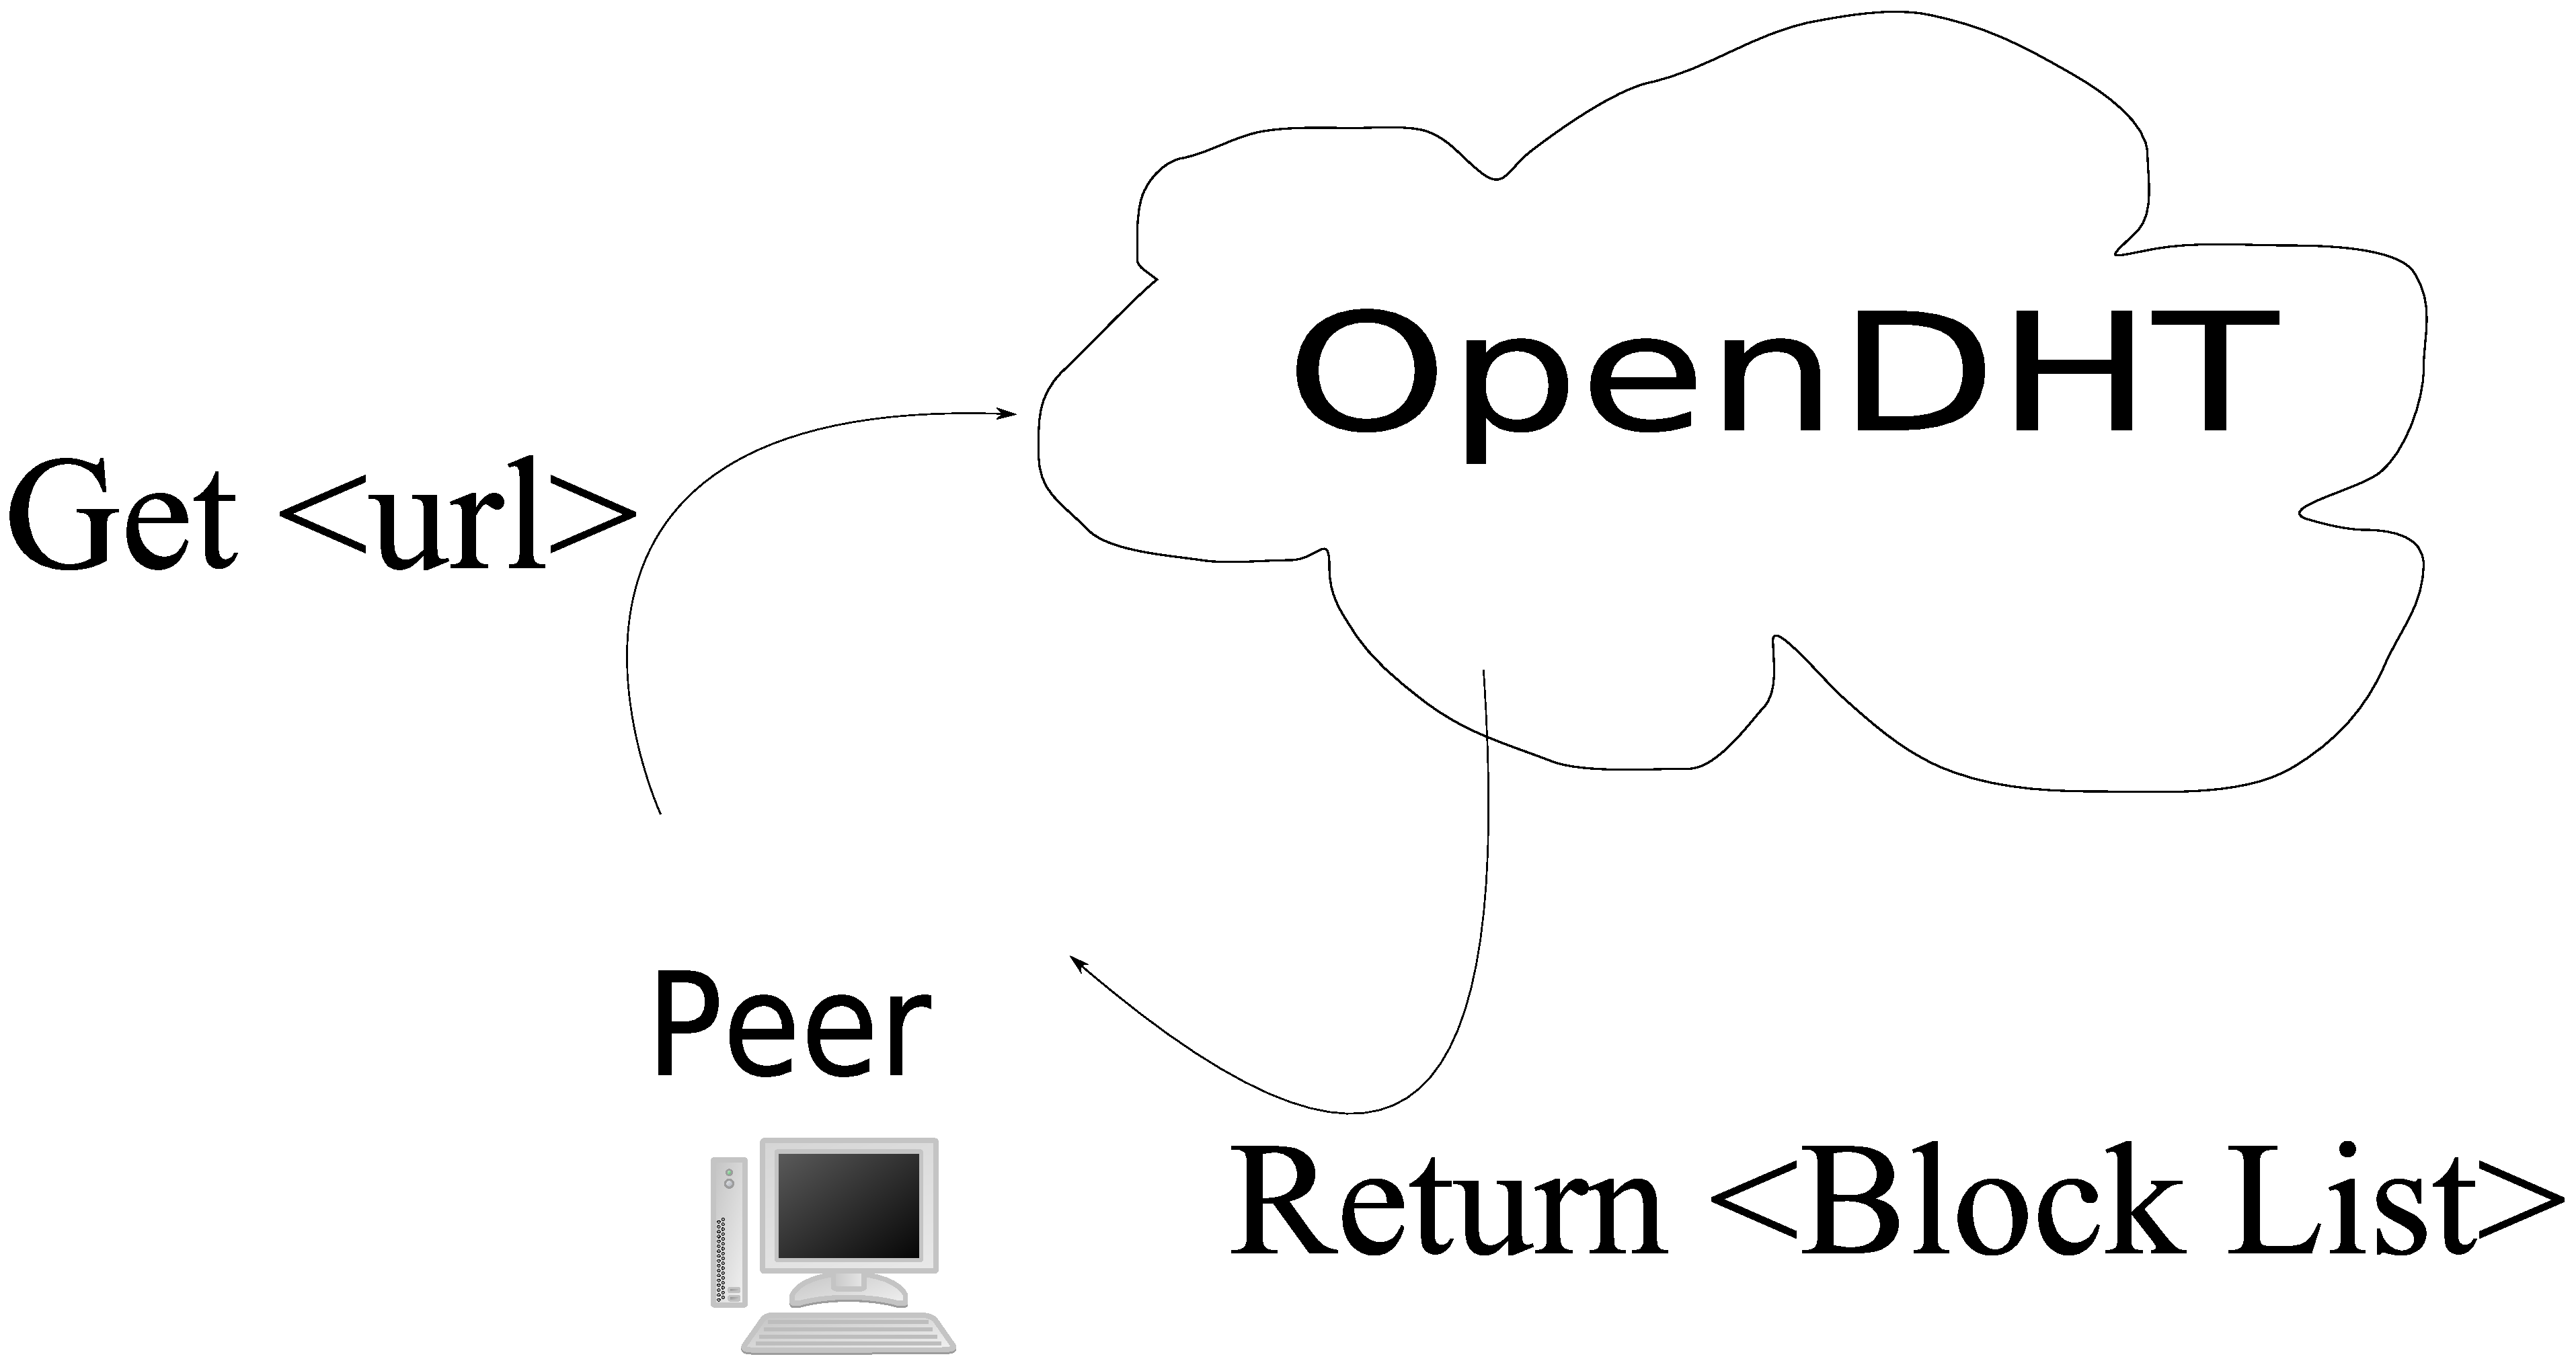
\includegraphics[width=7cm]{pics/peer_step_1.eps}}
    \subfigure[Peer downloads a list of peers which have a block]{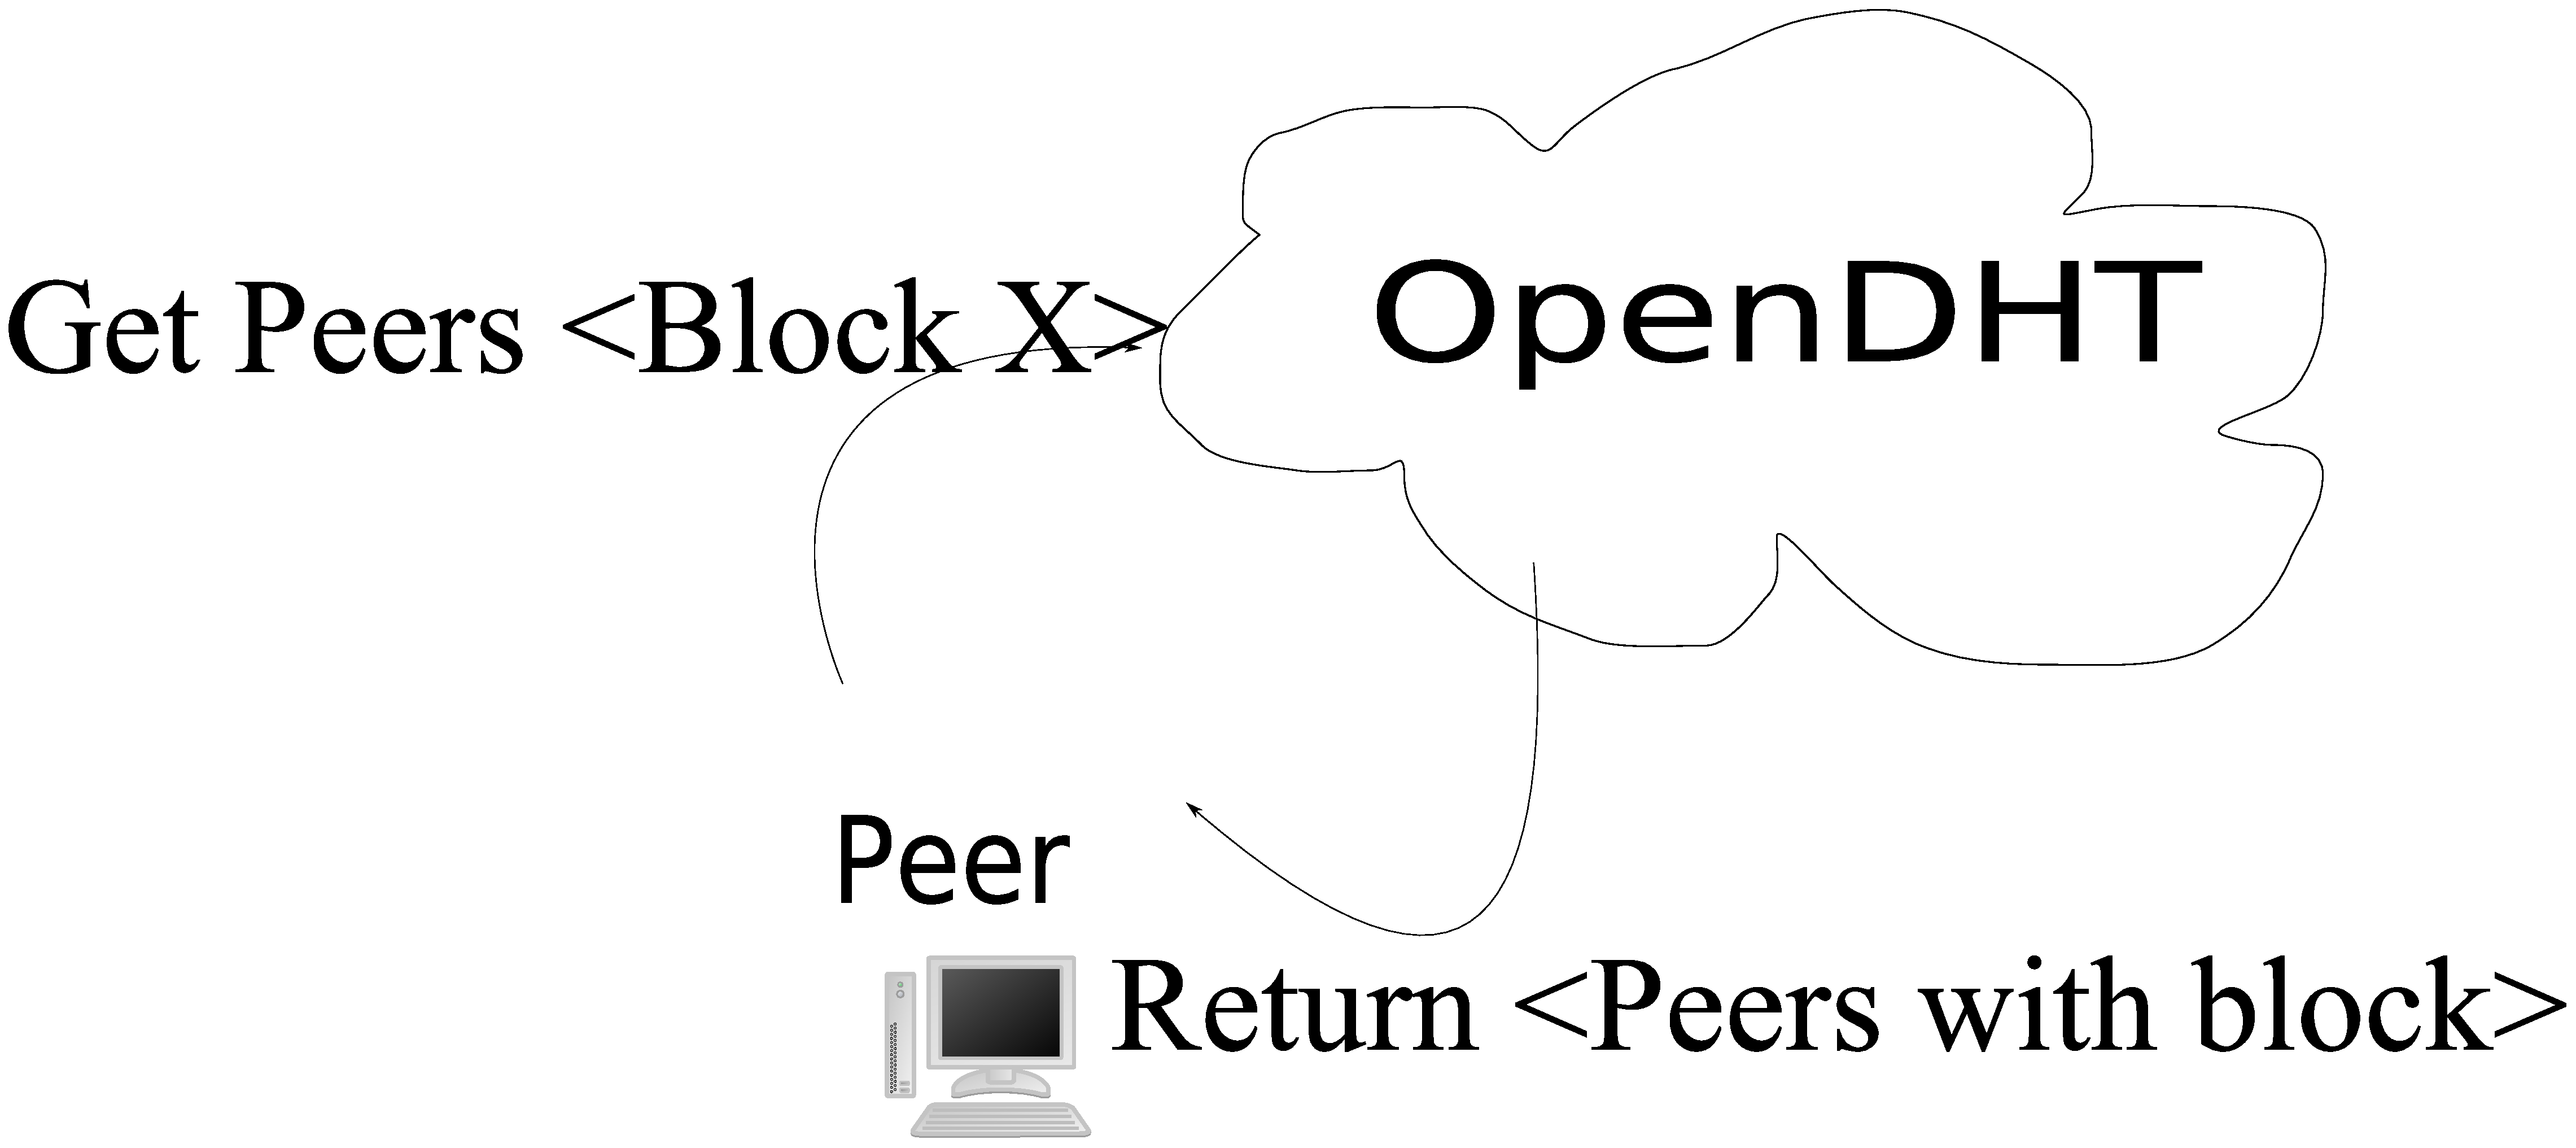
\includegraphics[width=7cm]{pics/peer_step_2.eps}}
    \subfigure[Peer adds itself to list of peers who have that block]{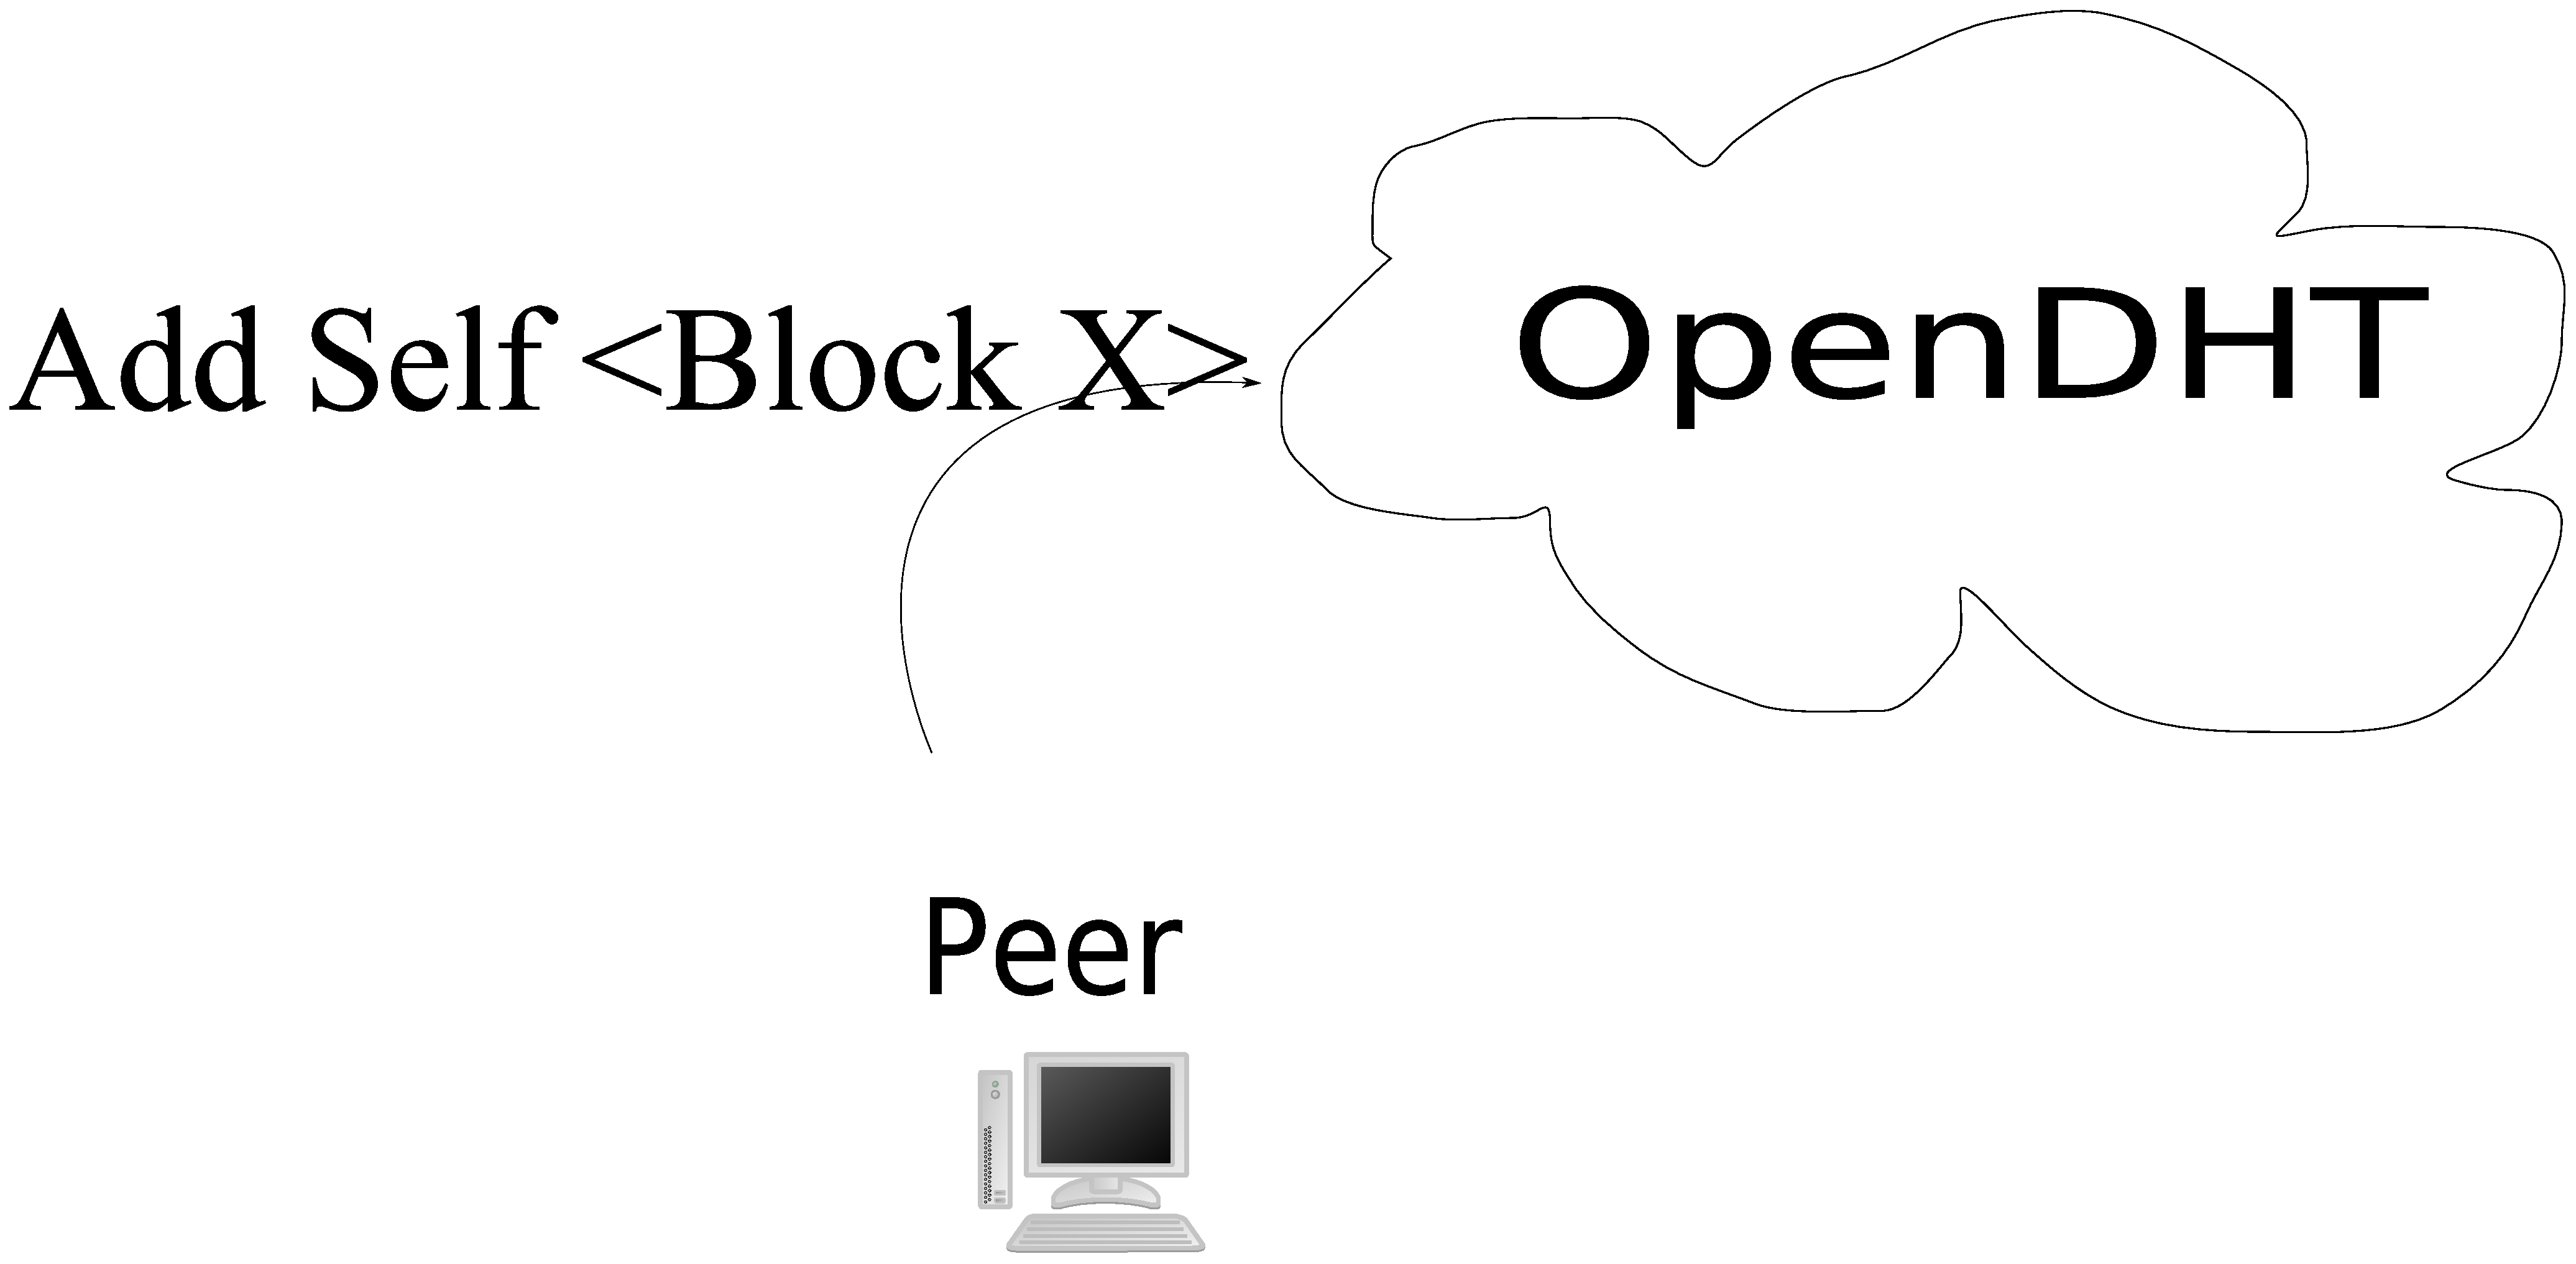
\includegraphics[width=7cm]{pics/peer_step_3.eps}}
    \caption{Steps to accomplish a peer-to-peer-web download.}
    \label{fig:download_all_steps}
  \end{center}
\end{figure*}

